\documentclass[10pt,a4paper]{article}
\usepackage[margin=0.8in,top=0.75in,bottom=0.75in]{geometry}
\usepackage[T1]{fontenc}
\usepackage{lmodern,microtype,amsmath,amssymb,booktabs,graphicx,xcolor,tikz,enumitem,array,multirow}
\newcolumntype{P}[1]{>{\raggedright\arraybackslash}p{#1}}
\usepackage[font=small,labelfont=bf,skip=3pt]{caption}
\usepackage[colorlinks=true,linkcolor=blue!50!black,citecolor=blue!50!black,urlcolor=blue!50!black]{hyperref}
\usetikzlibrary{positioning,arrows.meta,shapes.misc}
\setlist{nosep,leftmargin=1.3em}
\setlength{\parskip}{3pt}\setlength{\parindent}{0pt}
\renewcommand{\arraystretch}{1.08}
\newcommand{\best}[1]{\textbf{#1}}
\definecolor{teal}{HTML}{12968A}\definecolor{navy}{HTML}{0B132B}\definecolor{amber}{HTML}{F4B942}

\usepackage{float,needspace,etoolbox}
% keep headings with their content: never start a (sub)section in the last few lines of a page
\pretocmd{\section}{\Needspace{9\baselineskip}}{}{}
\pretocmd{\subsection}{\Needspace{7\baselineskip}}{}{}
\pretocmd{\subsubsection}{\Needspace{5\baselineskip}}{}{}
\hypersetup{pdftitle={Detector-Aware Data Augmentation for Network Intrusion Detection},pdfauthor={Aayush Majumdar and Vadiraj Rao}}
\setlength{\textfloatsep}{9pt}
\setlength{\intextsep}{9pt}
\raggedbottom
\begin{document}
\hypersetup{pageanchor=false}\begin{titlepage}
\centering\vspace*{2.2cm}
{\large CS5344 \quad|\quad Final Project Report}\\[1.2cm]
{\Huge\bfseries\color{navy} Detector-Aware Data Augmentation for Network Intrusion Detection}\\[0.4cm]
{\Large Shaping normal-only training data for fixed ECOD and Isolation Forest detectors on NSL-KDD and UNSW-NB15}\\[2cm]
{\Large \textbf{Group 42}}\\[0.6cm]
Aayush Majumdar \quad A0352046L\\
Vadiraj Rao \quad A0343563A\\[2cm]
National University of Singapore\\[0.3cm] November 2026
\end{titlepage}\setcounter{page}{1}\hypersetup{pageanchor=true}
\begin{abstract}\noindent
We generate normal-only training data for fixed ECOD and Isolation Forest detectors on two network-intrusion datasets. The supplied NSL-KDD and UNSW-NB15 tables contain 30\,000 and 50\,000 labeled records; the required outputs contain 40\,000 and 70\,000 normal records. Our objective is downstream attack-ranking utility rather than distributional fidelity. A shared pipeline combines configurable generation, category weighting, duplicate jitter, tail expansion, domain constraints, and feature neutralization. UNSW-NB15 benefits from contrastive normal reweighting and conditional Gaussian copulas with discriminative variance scaling. NSL-KDD benefits from retaining scrubbed normal observations and supplementing them with copulas fitted within SILK-style k-FreqItems clusters. On the public leaderboard, scores rise from 0.4210 to 0.61452 for UNSW-NB15 and from 0.92919 to 0.93734 for NSL-KDD. The selected submissions achieve final hidden AUPRC of \textbf{0.68508} and \textbf{0.95247}, respectively. Negative experiments show that additional generator complexity or stronger balancing does not reliably improve detector utility. We provide pseudocode, ablations, validation limitations, and lessons for reproducible distribution engineering.
\end{abstract}
\section{Introduction and Research Objectives}
Network-intrusion detection must distinguish legitimate traffic from attacks, including attack types absent from the supplied training data. Here the detector architecture is fixed: our intervention is the normal-only table on which it is trained. The task therefore asks whether changing normal coverage, category prevalence, and feature tails can improve detection without modifying the downstream models.

\textbf{Detector behavior.} ECOD~\cite{ecod} assigns outlier scores using empirical feature-tail probabilities. Isolation Forest~\cite{iforest} uses random feature splits: observations isolated through shorter paths receive higher anomaly scores. Both respond to the distribution of the submitted rows, although neither directly optimizes the attack labels available during augmentation.

\textbf{Evaluation objective.} Let $D=\{(x_i,y_i)\}_{i=1}^{n}$, where $y_i=1$ denotes an attack, and let $G_\theta(D)$ produce $m$ normal training rows. The optimization target is
\begin{equation}
\max_\theta S(\theta),\qquad
S=\tfrac12\left[\operatorname{AP}_{\rm ECOD}+\tfrac1{10}\sum_{r=1}^{10}\operatorname{AP}_{{\rm IF},r}\right].
\end{equation}
Average precision (AP), reported as AUPRC, weights precision by recall increments, $\sum_t(R_t-R_{t-1})P_t$; it summarizes ranking across thresholds rather than classification accuracy. Isolation Forest is evaluated over ten seeds with 500 trees per seed, as specified in the project protocol.

\textbf{Objectives and scope.} We seek to (i) improve both detectors through valid normal-data generation, (ii) support both mixed-attribute datasets through a common orchestration interface, and (iii) identify which transformations transfer across datasets. The two datasets use different generator and selector configurations behind the same interface.

\textbf{Contributions.} We present an empirical characterization of normal and attack regimes, two explicit generation configurations, a reproducible implementation, and an experimental analysis including unsuccessful approaches. The principal finding is that normal-distribution fidelity is insufficient as a standalone objective: useful transformations depend on both the data regime and the consuming detector.

\section{Dataset Characteristics and Exploratory Analysis}\label{sec:eda}
Both supplied datasets contain mixed numerical and categorical network records. NSL-KDD~\cite{nsl} describes connections through counts, rates, protocol/service fields, and content indicators. UNSW-NB15~\cite{unsw} describes flows through packet statistics, timings, TTLs, and connection state. Table~\ref{tab:data} gives the project subsets, rather than the full benchmark sizes.
\begin{table}[H]\centering\small
\begin{tabular}{lrrrp{2.8cm}rr}\toprule
Dataset & Train rows & Normal/attack & Feat. & Categorical (values) & Generate & Baseline AUPRC\\\midrule
UNSW-NB15 & 50\,000 & 35\,000/15\,000 & 42 & proto (86), service (13), state (8) & 70\,000 & 0.4210\\
NSL-KDD & 30\,000 & 20\,000/10\,000 & 41 & protocol (3), service (67), flag (11) & 40\,000 & 0.92919\\\bottomrule
\end{tabular}
\caption{Datasets. Baseline AUPRC is the public-leaderboard score of a bootstrap of the real normal rows.}\label{tab:data}
\end{table}
\paragraph{UNSW-NB15: heterogeneous traffic regimes.}
The bootstrap baseline is 0.4210. Across 118 protocol/service/state cells, observed attack shares range from 0.8\% in udp/dns/CON to 99\% in udp/dns/INT. Source TTLs 31 and 32 contain 64.8\% of normals and no observed attacks. Figure~\ref{fig:edau} motivates conditional generation and selective treatment of weak features.

\paragraph{NSL-KDD: strong empirical normal support.}
The baseline is 0.92919; 98.3\% of observed attacks have \texttt{logged\_\allowbreak in}=0, and flag S0 is 98\% attack. Several numerical columns have weak independent utility, while sparse content indicators may expose unseen attacks (Figure~\ref{fig:edan}). The design therefore retains normal modes, adds local variation, and protects sparse content features.

\textbf{Engineering implication.} UNSW motivates conditional redistribution; NSL-KDD motivates preservation. Both require explicit validity rules and evaluation of detector utility beyond marginal fidelity.
\begin{figure}[H]\centering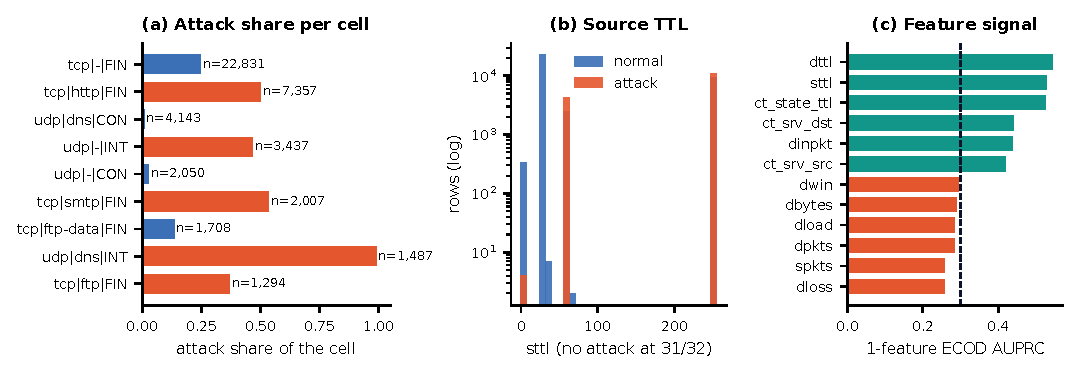
\includegraphics[width=0.94\linewidth]{../figs/eda_unsw.pdf}\caption{UNSW training diagnostics: attack share by traffic cell, source TTL, and single-feature ECOD utility; dashed utility line denotes attack prevalence.}\label{fig:edau}\end{figure}\begin{figure}[H]\centering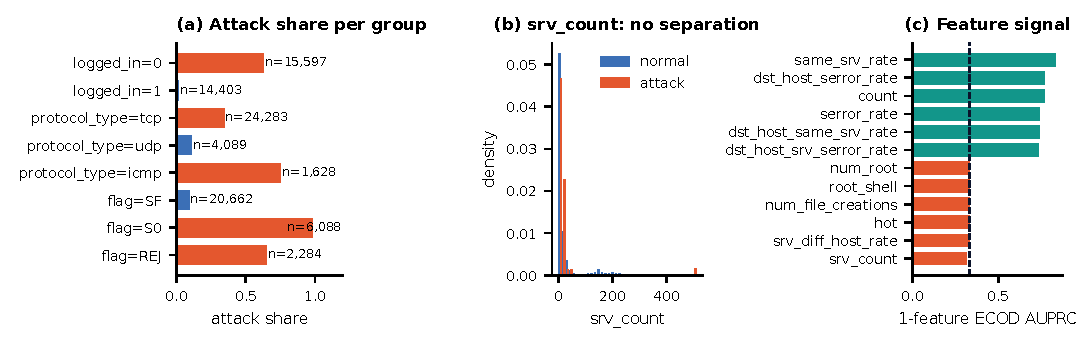
\includegraphics[width=0.94\linewidth]{../figs/eda_nsl.pdf}\caption{NSL-KDD training diagnostics: connection regimes, service-count overlap, and single-feature ECOD utility.}\label{fig:edan}\end{figure}

\section{Methodology}\label{sec:method}
\subsection{Shared Processing Architecture}
The pipeline separates statistical generation from common post-processing. Labeled inputs support normal extraction and utility estimation; attack rows inform selected transformations but are never exported as normal training records. Both configurations pass through the same functions (Figure~\ref{fig:pipe}), with neutral settings disabling irrelevant transformations.
\begin{figure}[H]\centering
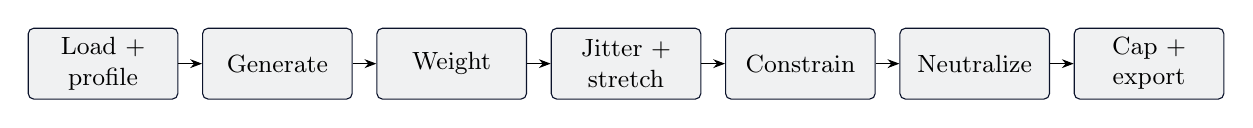
\begin{tikzpicture}[font=\small,node distance=3mm,
st/.style={draw=navy,fill=navy!6,rounded corners=2pt,minimum height=9mm,minimum width=19mm,align=center,inner sep=2pt}]
\node[st](a){Load +\\profile};\node[st,right=of a](b){Generate};
\node[st,right=of b](c){Weight};\node[st,right=of c](d){Jitter +\\stretch};
\node[st,right=of d](e){Constrain};\node[st,right=of e](f){Neutralize};
\node[st,right=of f](g){Cap +\\export};
\foreach\x/\y in {a/b,b/c,c/d,d/e,e/f,f/g}{\draw[-{Stealth[length=1.5mm]}](\x)--(\y);}
\end{tikzpicture}
\caption{Shared orchestration. NSL-KDD disables category weighting, duplicate jitter, and the separate tail-stretch stage. Local copula tail slack remains active.}\label{fig:pipe}
\end{figure}
\subsection{Common Statistical and Engineering Principles}
\textbf{Mixed attributes.} Categorical combinations are retained jointly rather than independently recombined. Numeric counts, bounded rates, binary indicators, and continuous measurements receive different treatment, preventing a continuous model from inventing fractional indicators or impossible protocol combinations.

\textbf{Conditional Gaussian copulas.} For a group $g$, each numerical variable is transformed through its empirical distribution and the standard normal inverse CDF:
\begin{equation}
u_{ij}=\widehat F_{gj}(x_{ij}),\quad z_{ij}=\Phi^{-1}(u_{ij}),\quad
\widetilde z\sim\mathcal N(0,R_g),\quad
\widetilde x_j=\widehat F_{gj}^{-1}\!\left(\Phi(\widetilde z_j)\right).
\end{equation}
This separates the shape of each marginal from dependence in Gaussian rank space. Correlation matrices are regularized to be positive definite; small groups borrow global correlation estimates.

\textbf{Feature neutralization.} A selected column is replaced independently across output rows by $U[Q_{0.01},Q_{0.99}]$, using quantiles of real normal observations; integer-valued columns are rounded. The bounds are the central 98\% interval of the normal data. A uniform density gives an approximately linear ECDF, which flattens the column's tail penalties in ECOD and prevents normal-tail clumping from causing shallow false-positive splits in Isolation Forest.

\begin{table}[H]\centering\small
\begin{tabular}{P{2.6cm}P{6.2cm}P{6.2cm}}\toprule
Component & UNSW-NB15 configuration & NSL-KDD configuration\\\midrule
Normal foundation & 35\,000 labeled normal rows; contrastive weighted resampling & 19\,600 normal rows after 2\% Isolation Forest scrub\\
Grouping & Joint protocol/service/state conditioning & SILK-style seeding and k-FreqItems refinement\\
Generation & 70\,000 DVS-copula rows; five sampling bags & 20\,400 local-copula rows plus all foundation rows\\
Main parameters & $\alpha=35$, $\tau_u=0.15$, $\tau_{low}=0.05$ & Selected $k=20$, $\rho=0.35$; later variant $18$, $0.30$\\
Resampling / tails & Weight scale 3; repeated-row jitter $0.10\sigma$; gated stretch 10 & Weight scale 0; jitter off; separate stretch factor 1\\
Neutralization & Four empirically selected columns & Six columns; sparse-content guard\\
Output & 70\,000 rows; schema and numeric checks & 40\,000 rows; schema and numeric checks\\\bottomrule
\end{tabular}
\caption{Configuration of the selected submissions; the later NSL-KDD variant is listed separately.}\label{tab:cfg}
\end{table}
\textbf{Design rationale.} Table~\ref{tab:cfg} contrasts the two configurations. The same interface exposes where the datasets differ: UNSW-NB15 requires substantial reweighting and dispersion, whereas NSL-KDD retains a strong empirical foundation. The following two subsections use the same five-part structure: preparation, grouping, generation, post-processing, and rationale.

\subsection{UNSW-NB15: Contrastive Conditional Copula Generation}
\subsubsection{Input Preparation and Feature Assessment}
The generator separates 35\,000 normal rows from 15\,000 attack rows and identifies categorical, integer-valued, and continuous columns. For each numerical feature $j$, ECOD is fitted on normal values and scores all labeled rows. Its utility is $c_j=\operatorname{Corr}(s_j^{\rm ECOD},y)$; the high-utility set is $H=\{j:c_j\ge0.15\}$.
\subsubsection{Grouping and Normal-Support Selection}
Contrastive purification favors normal observations whose useful feature values occur more often among normals than among attacks:
\begin{equation}
\ell_i=\sum_{j\in H}\log\frac{\widehat p_{0j}(x_{ij})+10^{-6}}{\widehat p_{1j}(x_{ij})+10^{-6}},\qquad
w_i=\frac{\exp(\operatorname{clip}(\ell_i,-10,10))}{\sum_l\exp(\operatorname{clip}(\ell_l,-10,10))}.
\end{equation}
The implementation uses empirical exact-value frequencies, with $10^{-4}$ for unseen values, and resamples 35\,000 normals with replacement using $w_i$. Purification is worth about $+0.07$ in the local harness and is a flat optimum around the default strength.

The final generator groups purified rows by joint \texttt{proto|service|state}. For a group of size $m_g$, $R_g^*=\lambda_gR_g+(1-\lambda_g)R_0$ with $\lambda_g=m_g/(m_g+100)$; groups below 50 rows use the global correlation. Jointly resampling categorical tuples avoids inventing unsupported combinations.
\subsubsection{Synthetic Sample Generation and Allocation}
Copula sampling reconstructs numerical marginals inside each regime. Discriminative variance scaling (DVS) then adds independent noise to eligible low-utility columns:
\begin{equation}
\widetilde x_{ij}\leftarrow\widetilde x_{ij}+\epsilon_{ij},\qquad
\epsilon_{ij}\sim\mathcal N\!\left(0,[35(0.05-c_j)_+\sigma_j]^2\right).
\end{equation}
Protected discrete indicators are excluded; other integer columns may be perturbed and then rounded. Expanded values are clipped from the observed normal minimum to $1.5$ times the positive normal maximum; high-utility and protected features retain observed bounds. Five seeded sampling bags of 14\,000 rows each produce 70\,000 rows. Dependence is modeled before perturbation, so DVS deliberately loosens it on weak columns.
\subsubsection{Post-processing and Domain Validation}
Category weights resample the pool with probability proportional to $\exp(3\theta_c)$, where $\theta_c$ is a per-cell log-weight fitted by an evolution strategy that maximizes the local-harness score over 14 protocol/service/state cells. Duplicate copies receive $0.10\sigma_j$ Gaussian jitter on eligible continuous features. A separate tail-stretch rule uses four attack clusters: a direction must meet AUC $0.58$ and agreement in at least 75\% of clusters; the opposite normal tail is stretched tenfold about its 10th or 90th percentile. For example, if attacks are consistently low, an upper-tail value becomes $x'=Q_{0.90}+10(x-Q_{0.90})$.

Domain rules enforce non-negativity, integer counts, TTL bounds, protocol-specific zeroing, and TCP timing consistency. Uniform filling replaces \texttt{sinpkt}, \texttt{sjit}, \texttt{ct\_\allowbreak dst\_\allowbreak src\_\allowbreak ltm}, and \texttt{ct\_\allowbreak dst\_\allowbreak ltm}; final caps constrain selected counts to 100 and \texttt{dmean} to 1500. Constraints repair invalid values, while neutralization changes detector sensitivity.
\subsubsection{Rationale and Expected Detector Effect}
Conditioning avoids averaging unrelated traffic regimes; purification changes which normal modes dominate training; DVS widens weak dimensions so they stop producing false alarms; tail stretching widens the normal side that attacks do not occupy. Each benefit was established empirically on the leaderboard (Section~\ref{sec:exp}).

\subsection{NSL-KDD: Mixed-Attribute Clustering and Local Copula Generation}
\subsubsection{Input Preparation and Feature Assessment}
Isolation Forest removes the most readily isolated 2\% of 20\,000 normal observations, leaving a 19\,600-row foundation that is preserved through generation (later constraints and neutralization still apply). Binary and low-cardinality integer features remain exact; continuous variables are discretized into up to five quantile bins, with duplicate quantile edges collapsed.
\subsubsection{Grouping and Normal-Support Selection}
A row becomes an itemset such as $\{\texttt{protocol=tcp},\texttt{service=http},\texttt{src\_\allowbreak bytes=q3},\ldots\}$; an item is a feature--value token, not an entire record. Five bins give a coarse ordinal representation while avoiding excessive sparsity. Figure~\ref{fig:silk} summarizes the clustering stage.
\begin{figure}[H]\centering
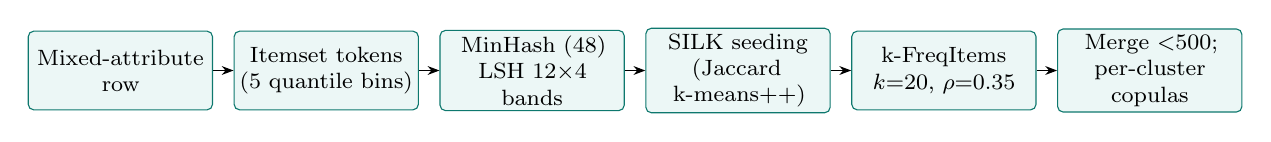
\begin{tikzpicture}[font=\footnotesize,node distance=2.6mm,
st/.style={draw=teal!80!black,fill=teal!8,rounded corners=2pt,minimum height=10mm,text width=22mm,align=center,inner sep=2pt}]
\node[st](a){Mixed-attribute\\row};
\node[st,right=of a](b){Itemset tokens\\(5 quantile bins)};
\node[st,right=of b](c){MinHash (48)\\LSH 12$\times$4 bands};
\node[st,right=of c](d){SILK seeding\\(Jaccard k-means++)};
\node[st,right=of d](e){k-FreqItems\\$k{=}20$, $\rho{=}0.35$};
\node[st,right=of e](f){Merge ${<}500$;\\per-cluster copulas};
\foreach\x/\y in {a/b,b/c,c/d,d/e,e/f}{\draw[-{Stealth[length=1.5mm]}](\x)--(\y);}
\end{tikzpicture}
\caption{NSL-KDD clustering. Hashing only proposes seeds; assignment and centre updates use the original token sets and Jaccard distance.}\label{fig:silk}
\end{figure}
MinHash~\cite{minhash} maps each set to 48 minimum-hash values using deterministic FNV-style token hashing and seeded affine modular transforms. LSH splits this signature into 12 bands of four values and collects identical bands into candidate buckets. SILK-style seeding constructs frequent-token candidate centres and selects separated candidates with probability proportional to bucket weight times squared distance, adapting k-means++~\cite{kmpp} to Jaccard distance:
\begin{equation}
d_J(A,B)=1-\frac{|A\cap B|}{|A\cup B|},\qquad
C_j=\left\{t:\frac{\#\{i\in I_j:t\in R_i\}}{|I_j|}\ge\rho\right\}.
\end{equation}
K-FreqItems alternates nearest-centre assignment and frequency-centre updates until assignments stabilize or 25 iterations are reached. The selected configuration uses $k=20$, $\rho=0.35$; the later $k=18$, $\rho=0.30$ variant uses the same procedure. Here $\rho$ is within-cluster item frequency, not association-rule confidence. Clusters below 500 rows merge into the nearest sufficiently large cluster, so the final number can be below $k$. The procedure is SILK-inspired rather than a full reproduction of the published algorithm.
\subsubsection{Synthetic Sample Generation and Allocation}
For cluster $j$ with $n_j$ foundation rows, its additional-row budget is
\begin{equation}
a_j=20\,400\frac{n_j}{19\,600}.
\end{equation}
Floors are assigned first; remaining rows go to the largest fractional remainders, with deterministic label tie-breaking. Each sufficiently large cluster has two seeded, protocol-conditioned copula models; global models provide a fallback. A tail-slack factor of 1.05 mildly expands eligible continuous upper tails while bounded rates remain protected. Thus 19\,600 foundation rows plus 20\,400 generated rows produce exactly 40\,000 records before post-processing.
\subsubsection{Post-processing and Domain Validation}
Separate category weighting, duplicate jitter, and gated tail stretching are disabled. Constraints enforce rates in $[0,1]$, non-negative integer counts, and valid indicators. Six columns receive uniform fill: \texttt{srv\_\allowbreak count}, \texttt{srv\_\allowbreak diff\_\allowbreak host\_\allowbreak rate}, \texttt{duration}, \texttt{dst\_\allowbreak host\_\allowbreak count}, \texttt{dst\_\allowbreak host\_\allowbreak same\_\allowbreak src\_\allowbreak port\_\allowbreak rate}, and \texttt{dst\_\allowbreak host\_\allowbreak rerror\_\allowbreak rate}. Selection uses single-feature AP lift above attack prevalence of at most 0.10, protects columns with a dominant value share of at least 0.90, and excludes \texttt{dst\_\allowbreak host\_\allowbreak srv\_\allowbreak diff\_\allowbreak host\_\allowbreak rate} after an adverse experiment.
\subsubsection{Rationale and Expected Detector Effect}
The real-normal baseline is already strong, so proportional local synthesis adds variation without equalizing rare and common modes. Itemsets accommodate categories and discretized measurements in one similarity measure, avoiding Euclidean coding assumptions for categorical fields.

\section{Implementation and Reproducibility}\label{sec:impl}
\subsection{Code Organization and Artifact Flow}
\texttt{pipeline.py} loads configuration, dispatches a generator, applies transformations, and writes ordered CSV columns with unique IDs (Figure~\ref{fig:algorithm}). \texttt{config.py} stores target sizes, seeds, generator choices, selector settings, and artifact paths. The \texttt{modules} package contains DVS, SILK-style clustering, the hybrid allocator, copula sampling, and domain constraints. The experiment scripts behind Section~\ref{sec:exp}, including the local harness and all leaderboard variants, are in the project repository (\url{https://github.com/jeet30/CS5344_BDT_project}).

The NSL foundation CSV, category weights, and feature-selection tables are persisted artifacts. Reusing them makes runs exactly reproducible, but the export command is not a fresh end-to-end refit of every upstream decision; each result is therefore tied to a configuration and data snapshot.
\begin{figure}[H]\centering
\fbox{\begin{minipage}{0.94\linewidth}\small
\textbf{Algorithm 1: Configurable normal-data generation and export}\\[-2pt]
\rule{\linewidth}{0.4pt}
\textbf{Input:} labeled data $D$, configuration $\theta$, saved artifacts $A$, target $m$, seed $s$.\\
\textbf{Output:} normal-only table $S$ with $m$ records and ordered feature columns.
\begin{enumerate}[label=\arabic*.,leftmargin=2em,itemsep=3pt]
\item Load $D$; separate labels, categorical columns, and numerical columns.
\item \textbf{If} the generator is contrastive DVS:
  estimate feature utility; reweight normals; fit conditional copulas; sample $m$ rows; apply selective dispersion.
\item \textbf{Otherwise, if} the generator is the SILK hybrid:
  load the scrubbed foundation; tokenize; form MinHash--LSH candidates; choose seeds; refine k-FreqItems clusters; allocate $m-|D_0|$ rows proportionally; sample local copulas; combine with $D_0$.
\item Apply configured category-cell weights by sampling with replacement.
\item Jitter repeated rows on eligible continuous columns when enabled.
\item Estimate consistent attack directions and stretch opposite normal tails when enabled.
\item Enforce dataset domain rules; replace selected weak columns using normal quantile bounds; apply final hard caps.
\item Restore feature order; add unique IDs; assert row count, no missing values, and unique IDs; export CSV.
\item Compare against a reference artifact when available; record configuration and diagnostics for interpretation.
\end{enumerate}
\end{minipage}}
\caption{Implementation-level pseudocode matching the shared transformation order. Neutral parameters disable optional stages; reference comparison is a separate verification operation.}\label{fig:algorithm}
\end{figure}
\subsection{Computational Characteristics and Validation Boundaries}
With $n$ rows, $d$ tokens per row, and $h=48$ hashes, signature construction costs $O(ndh)$. Direct Jaccard assignment is approximately $O(Tnkd)$ for $T\le25$ iterations and bounded-size centres. LSH reduces seed-search work but does not replace these full assignment passes. Copula covariance estimation scales as $O(nd^2)$ and matrix factorization as $O(d^3)$ per fitted group; small-group regularization is important for numerical stability.

The implementation uses pandas/NumPy, SciPy, scikit-learn, and PyOD in an in-memory Python workflow; both datasets export in seconds. We did not measure distributed speedup, so scalability claims are limited to these algorithmic costs. Larger deployments would require profiling, batched signatures, and group-parallel fitting.

\textbf{Audit scope.} Export assertions cover row count, unique IDs, and missing values. Finite-value and cross-feature domain checks are recommended additional release checks, because neutralization follows constraints. \texttt{verify.py} reproduces the scored files to within $10^{-9}$.

\section{Experimental Design and Comparative Results}\label{sec:exp}
\subsection{Evaluation Protocol and Score Provenance}
Two evaluation sources are used. The \emph{public leaderboard} scored submissions during development on a 39\% subset of the test data (seen and validation attack types); all ablations below use it. The \emph{final hidden leaderboard} rescored the selected submissions on the full test set after the hidden data were revealed; it includes at least one attack type absent from both training and the public subset, and is on a different scale. Hidden scores are therefore higher in absolute terms but must not be subtracted from public scores to infer an improvement. A 14-fold local harness simulated distribution shifts through held-out attack clusters, categorical groups, and tail regions; it screened candidates but did not reliably reproduce leaderboard rankings.

\subsection{Cumulative Improvements on Both Datasets}
\begin{figure}[H]\centering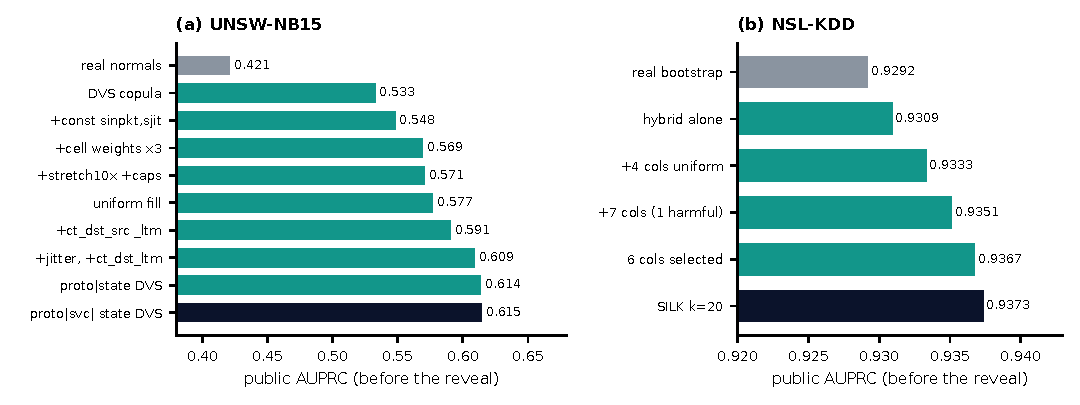
\includegraphics[width=0.94\linewidth]{../figs/journey.pdf}\caption{Public-leaderboard progression for the two datasets. These are method comparisons, not precision--recall curves.}\label{fig:journey}\end{figure}\begin{table}[H]\centering\small
\begin{tabular}{p{7.8cm}rr}\toprule
Step (UNSW-NB15) & Public AUPRC & $\Delta$\\\midrule
Bootstrap of real normals & 0.4210 & --\\
Contrastive DVS copula, proto-conditioned & 0.53263 & +0.11163\\
+ stability-gated constants (\texttt{sinpkt}, \texttt{sjit}) & 0.54803 & +0.01540\\
+ $6\times$ gated tail stretch & 0.55048 & +0.00245\\
+ cell weights $\times1/\times2/\times3/\times4$ & 0.55468/0.56254/\best{0.56940}/0.56106 & +0.01892\\
$10\times$ stretch with physical caps & 0.57067 & +0.00127\\
uniform instead of constant fill & 0.57698 & +0.00631\\
+ \texttt{ct\_\allowbreak dst\_\allowbreak src\_\allowbreak ltm} filled (selection re-run) & 0.59066 & +0.01368\\
+ duplicate jitter, + \texttt{ct\_\allowbreak dst\_\allowbreak ltm} (selection round 2) & 0.60905 & +0.01839\\
50/50 blend of proto- and state-conditioned DVS & 0.61316 & +0.00411\\
single DVS on joint proto$|$state & 0.61392 & +0.00076\\
\best{single DVS on joint proto$|$service$|$state} & \best{0.61452} & +0.00060\\\bottomrule
\end{tabular}
\caption{UNSW-NB15 cumulative ablation (public leaderboard). Each $\Delta$ is relative to the previous row; the weight row uses $\times3$.}\label{tab:uns}\end{table}\begin{table}[H]\centering\small
\begin{tabular}{p{9.5cm}rr}\toprule
Step (NSL-KDD) & Public AUPRC & $\Delta$\\\midrule
Bootstrap of real normals & 0.92919 & --\\
Hybrid (real + itemset-cluster copulas) alone & 0.93092 & +0.00173\\
+ 4 uniform-filled columns & 0.93331 & +0.00239\\
+ 7 columns (includes one harmful column) & 0.93512 & +0.00181\\
6 columns (harmful column removed) & 0.93674 & +0.00162\\
\best{SILK-seeded k-FreqItems clusters instead of itemset clusters} & \best{0.93734} & +0.00060\\\bottomrule
\end{tabular}
\caption{NSL-KDD cumulative ablation (public leaderboard).}\label{tab:nsl}\end{table}
\textbf{Interpretation.} Figure~\ref{fig:journey} and Tables~\ref{tab:uns}--\ref{tab:nsl} trace both progressions. UNSW gains 0.19352 over its baseline, primarily from contrastive DVS (+0.11163) and the post-processing stack. NSL-KDD gains 0.00815, mostly through feature neutralization (+0.00582 across the fill rows).

\Needspace{0.45\textheight}
\subsection{Sensitivity Analysis and Unsuccessful Alternatives}
Negative experiments delimit the useful configuration space (Table~\ref{tab:neg}). Values shown at fewer than five decimals were recorded at that precision.
\begin{table}[H]\centering\small
\begin{tabular}{P{3.3cm}P{1.45cm}P{1.45cm}P{8.0cm}}\toprule
Experiment & NSL-KDD & UNSW-NB15 & Interpretation\\\midrule
CTGAN~\cite{ctgan} & 0.9215 & 0.3925 & Below the bootstrap baseline on both datasets: fidelity-oriented generation did not preserve detector-relevant tails or sparse categories\\
Global clustering + copula & 0.9281 & 0.4397 & Cluster objective misaligned with detector utility\\
Density-ratio rejection & 0.9279 & 0.4925 & Hard rejection contracts the normal support\\
DVS purification applied to NSL-KDD & $\approx$0.899 & -- & Over-purifies normals that are already strong; NSL needs preservation\\
Constant fill of 11 columns (NSL) & 0.91799 & -- & Froze informative columns (\texttt{service}, \texttt{logged\_\allowbreak in}); the sparse-support guard prevents this\\
Category weights up/down (NSL) & 0.92197/\allowbreak 0.92901 & -- & Weights on service/flag distort useful normal proportions; no signal lever\\
Log-uniform fill (NSL) & 0.93101 & -- & $-0.00573$ vs raw-scale uniform (0.93674); compresses the range the detector sees\\
Filling \texttt{dst\_\allowbreak host\_\allowbreak srv\_\allowbreak \allowbreak diff\_\allowbreak host\_\allowbreak rate} (NSL) & 0.93192 & -- & Adding it to the 4-column set lost 0.00139; removing it from the 7-column set gained 0.00162, although its single-feature lift is only 0.036\\
(protocol, flag) partition (NSL) & 0.93642/\allowbreak 0.93668 & -- & Mixed with SILK / alone: no gain over SILK (0.93734)\\
No duplicate rows (16$\times$ pool, no replacement) & -- & 0.56630 & $-0.00437$ vs 0.57067: sampling with replacement keeps more mass on useful cells\\
40-cell weights fitted on a different base & -- & 0.59394 & $-0.02058$ vs 0.61452: harness gain did not transfer (Table~\ref{tab:har})\\
Extra $\times0.5$ on four shared cells & -- & 0.59746 & $-0.01706$: both directions lose; the 14-cell optimum is sharp\\
Three-way mix (proto, state, SILK) & -- & 0.60781 & More than two partitions is worse than one or two\\
65\% state-conditioned DVS & -- & 0.6097 & Increasing the state-conditioned share lowered the score\\\bottomrule
\end{tabular}
\caption{Negative results (public leaderboard AUPRC).}\label{tab:neg}\end{table}\begin{figure}[H]\centering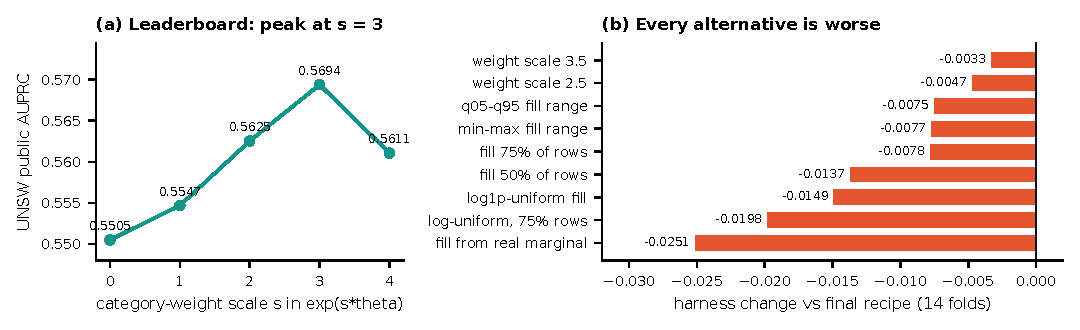
\includegraphics[width=\linewidth]{../figs/sensitivity.pdf}\caption{UNSW sensitivity: leaderboard performance by weight scale (left) and local-harness changes for alternative fill rules (right). The panels use different evaluation sources.}\label{fig:sens}\end{figure}
\textbf{Implication.} Figure~\ref{fig:sens} shows the same pattern for UNSW: the weight scale peaks at 3, and every alternative fill rule loses in the harness. More balancing, stronger dispersion, or finer conditioning can change useful normal prevalence as well as coverage, and their effect depends on the rest of the configuration. A failed variant rejects that tested configuration, not the underlying model family.

\Needspace{14\baselineskip}
\subsection{Final Scores}
Table~\ref{tab:final} reports the selected submissions and their final hidden scores. Only the best pre-reveal files were eligible for selection; two later parameter variants are listed separately for completeness.
\begin{table}[H]\centering\small
\begin{tabular}{P{3.0cm}P{7.2cm}P{2.6cm}P{1.6cm}}\toprule
Dataset / record & Configuration & Evaluation & AUPRC\\\midrule
UNSW selected & Joint proto/service/state DVS & Final hidden & \best{0.68508}\\
NSL selected & SILK $k=20$, frequency 0.35 & Final hidden & \best{0.95247}\\
UNSW later variant & \texttt{submission\_\allowbreak unsw\_\allowbreak v2\_\allowbreak state35.csv} & Final hidden, not selected & 0.68651\\
NSL later variant & \texttt{submission\_\allowbreak nslkdd\_\allowbreak v2\_\allowbreak k18\_\allowbreak cf30.csv} & Final hidden, not selected & 0.95276\\\bottomrule
\end{tabular}
\caption{Final hidden scores. Later variants were not the selected submissions; no matched causal comparison is asserted.}\label{tab:final}
\end{table}
\subsection{Local Validation Reliability and Residual Errors}
\begin{table}[H]\centering\small
\begin{tabular}{P{6.6cm}P{3.7cm}P{3.1cm}}\toprule
Decision & Harness prediction & Leaderboard\\\midrule
40-cell category weights vs 14-cell & +0.0069 held-out (+0.0172 in-sample) & $-0.02058$\\
UNSW uniform vs constant fill of \texttt{sinpkt}, \texttt{sjit} & +0.0023 & +0.00631\\
\texttt{ct\_\allowbreak dst\_\allowbreak ltm} added to the filled columns & +0.0037 & +0.00123\\
Duplicate-row jitter ($0.10\sigma$) & +0.0057 & +0.01108\\
50\% proto + 50\% state vs proto-only generator & no difference (0.5704 both) & +0.00411\\
NSL-KDD: hold \texttt{srv\_\allowbreak count}, \texttt{srv\_\allowbreak diff\_\allowbreak host\_\allowbreak rate} constant & $-0.003$ / $-0.0014$ & +0.00087\\
NSL-KDD: log-uniform fill & ($-0.0149$ on UNSW) & $-0.00573$\\\bottomrule
\end{tabular}
\caption{Harness vs.\ leaderboard on individual decisions; harness values recorded at 4 dp. Leaderboard deltas are measured against the file each decision modified (e.g.\ jitter against 0.57698, \texttt{ct\_\allowbreak dst\_\allowbreak ltm} against 0.60782), so they differ from the cumulative rows of Table~\ref{tab:uns}.}\label{tab:har}\end{table}\begin{figure}[H]\centering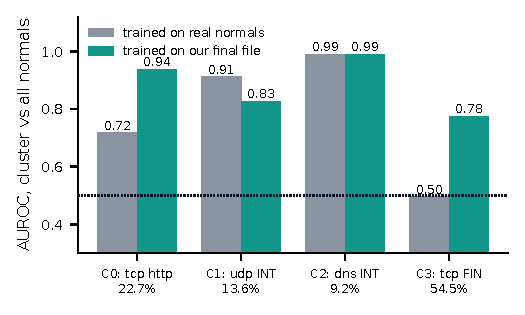
\includegraphics[width=0.50\linewidth]{../figs/clusters.pdf}\caption{UNSW in-sample attack-cluster AUROC, with detectors trained on baseline versus generated normals (AUROC, not AUPRC).}\label{fig:clu}\end{figure}
Table~\ref{tab:har} compares harness predictions with leaderboard outcomes. Per attack cluster (Figure~\ref{fig:clu}), the generated UNSW distribution improves the large TCP cluster from AUROC 0.496 to 0.775 but lowers the UDP cluster from 0.913 to 0.827, so aggregate gains can conceal regressions on individual attack regimes. A supervised diagnostic reaches 0.971 in the difficult TCP cell, while unsupervised views top out near 0.75--0.80, suggesting that joint discriminative structure remains underused by the fixed detectors.

\textbf{Threats to validity.} (i) Seed variance was not measured, so leaderboard deltas below about 0.002 (e.g.\ the final +0.00060 steps) are indicative only. (ii) Repeated public-leaderboard tuning creates selection bias. (iii) Cumulative ablations do not isolate causal contributions; our mechanisms for tail shaping, purification, and uniform fill are plausible, not measured. (iv) Feature utilities $c_j$ and the cluster AUROCs are in-sample. (v) Purification may suppress legitimate rare normal regimes, and DVS and neutralization deliberately break some learned dependence. (vi) Only scalar hidden scores exist, so hidden PR curves cannot be drawn.

\section{Lessons Learned}\label{sec:lessons}
\paragraph{1. Shape the data for the detector, not for fidelity.}
CTGAN, the most fidelity-oriented generator, scored 0.3925 on UNSW, \emph{below} the 0.4210 bootstrap of real normals, while the detector-aware DVS pipeline reached 0.61452. Deliberately unrealistic choices won repeatedly: uniform fill beat constant fill (0.57698 vs 0.57067), and a fill drawn from the real marginal was the worst harness option ($-0.0251$, 0 of 14 folds improved). Validity, support coverage, and detection utility must be assessed separately.

\paragraph{2. Dataset structure determines which transformations are useful.}
NSL-KDD's strong real-normal baseline favors preservation and modest local synthesis; UNSW's heterogeneous traffic cells support conditional generation and extensive redistribution. Transferring aggressive purification to NSL-KDD reduced its score to approximately 0.899, and category weights are a $\pm0.02$ lever on UNSW but empty on NSL-KDD. A shared interface with neutral parameters let one pipeline serve both.

\paragraph{3. Local models require sufficient support and regularization.}
Conditioning improved UNSW incrementally (proto 0.60905 $\to$ proto$|$state 0.61392 $\to$ proto$|$service$|$state 0.61452), while small-cluster merging and correlation shrinkage kept copula fitting stable. More mixture components did not help (three-way mix 0.60781). Group size, fallback behavior, and locality matter more than the number of clusters.

\paragraph{4. Proxy validation can mis-rank promising changes.}
Forty-cell weights improved the held-out harness by 0.0069 but reduced the public score by 0.02058; the NSL harness predicted the opposite sign for neutralizing \texttt{srv\_\allowbreak count}. We therefore stopped using the harness for NSL decisions and used it only to screen UNSW candidates, judging close calls on the leaderboard.

\paragraph{5. Change one thing at a time.}
Because the leaderboard was the final arbiter, we built one-change A/B files that hold every other random draw fixed (e.g.\ skipping one filled column leaves all other values identical). This isolated the harmful \texttt{dst\_\allowbreak host\_\allowbreak srv\_\allowbreak diff\_\allowbreak host\_\allowbreak rate} column ($-0.00139$ when added, $+0.00162$ when removed). Future work should add generation-seed repeats and bootstrap intervals to this protocol.

\paragraph{6. Check intuitive explanations with a direct test.}
After 40-cell weights that upweighted attack-overlapping cells lost 0.02058, we inferred that downweighting those cells should help; it lost 0.01706. Both directions failing showed the 14-cell weights were a sharp optimum and our explanation was wrong. Similarly, cluster-level diagnostics revealed the UDP regression hidden by the aggregate gain. Per-regime false-positive and recall measurements should accompany aggregate AUPRC.

\section{Conclusion and Future Work}
The project demonstrates a configurable workflow for generating valid normal-only training tables for fixed anomaly detectors. Public-leaderboard improvements were substantial on UNSW-NB15 and smaller on NSL-KDD, reflecting different starting distributions. Conditional contrastive copulas and selective dispersion served UNSW; preserving normal observations and generating within mixed-attribute clusters served NSL-KDD. The evidence supports empirical configuration selection, not a universal superiority claim for clustering or DVS. Future work should use nested selection for weights and feature filling, measure seed uncertainty, test restoration of suppressed normal regimes, and profile batched or parallel group fitting before making large-scale deployment claims.

\paragraph{Reproducibility and AI use.}
The source code for all experiments (generators, local harness, ablations, and leaderboard variants) is available at \url{https://github.com/jeet30/CS5344_BDT_project}. The accompanying submission contains only the final-pipeline reproduction (\texttt{Group42Codebase}): \texttt{python pipeline.py unsw} or \texttt{nslkdd} regenerates the selected files, and \texttt{verify.py} checks them against the scored references using the shipped artifacts and pinned dependencies. Claude (Anthropic) and OpenAI Codex assisted with code, analysis and editing; the authors verified all methods and results.

\clearpage
\begin{thebibliography}{9}\small
\bibitem{ecod} Z.~Li, Y.~Zhao, X.~Hu, N.~Botta, C.~Ionescu, G.~Chen. ECOD: Unsupervised outlier detection using empirical cumulative distribution functions. \emph{IEEE TKDE}, 2022. \url{https://doi.org/10.1109/TKDE.2022.3159580}.
\bibitem{iforest} F.~T.~Liu, K.~M.~Ting, Z.-H.~Zhou. Isolation Forest. \emph{IEEE ICDM}, 2008.
\bibitem{nsl} M.~Tavallaee, E.~Bagheri, W.~Lu, A.~A.~Ghorbani. A detailed analysis of the KDD CUP 99 data set. \emph{IEEE CISDA}, 2009.
\bibitem{unsw} N.~Moustafa, J.~Slay. UNSW-NB15: A comprehensive data set for network intrusion detection systems. \emph{MilCIS}, 2015.
\bibitem{ctgan} L.~Xu, M.~Skoularidou, A.~Cuesta-Infante, K.~Veeramachaneni. Modeling tabular data using conditional GAN. \emph{NeurIPS}, 2019. \url{https://arxiv.org/abs/1907.00503}.
\bibitem{minhash} A.~Z.~Broder. On the resemblance and containment of documents. \emph{SEQUENCES}, 1997.
\bibitem{kmpp} D.~Arthur, S.~Vassilvitskii. k-means++: The advantages of careful seeding. \emph{SODA}, 2007.
\end{thebibliography}
\end{document}
